\section{Profunctors / Grothendieck construction}
\label{sec:org7dd09e1}
There are two possible ways to define a relation $R$ between two sets $A,B$:
\begin{enumtag}{r}
	\item \label{r_1} a relation $R$ is a subset of the cartesian product $A\times B$;
	\item \label{r_2} a relation $R$ is a function $A\times B \to \{0,1\}$.
\end{enumtag}
Note that the notion of `relation between $A$ and $B$' is inherently symmetric, in the sense that such $R$ can be regarded both as a relation `from' $A$ `to' $B$, and as a relation `from' $B$ `to' $A$.

Furthermore, every relation $R$ between sets $A,B$ gives rise to a \emph{Galois connection}
\[{}^R(\firstblank) :PA^\op \leftrightarrows PB : (\firstblank)^R \label{adjunzia} \]
between the powersets $PA=2^A$ and $PB = 2^B$: the set $U\subset A$ goes to the set ${}^RU$ of all $b$ such that $(a,b)\in R$ for all $a\in U$; in an exactly symmetric way, a set $V\subseteq B$ goes to the set
\[V^R = \{a\in A\mid (a,b) \in R,\, \forall b\in V\}.\]
Unwinding the definition, it is asy to verify that $V\subseteq{}^RU$ if and only if $U\subseteq V^R$, if and only if $U\times V\subseteq R$.
%\todo[inline]{La varianza di sta roba va controllata}

From here, using a process known as `categorification' \cite{baez_catego}, we can replace a two-valued relation $R : A\times B \to \{0,1\}$ with a \emph{set-valued} functor $\clA^\op\times\clB \to \Set$ between two (small) categories $\clA,\clB$.\footnote{The reason why the category $\clA$ is twisted with an `$^\op$' functor is that we want to bestow the hom functor $\hom_{\clA} : \clA^\op\times\clA \to \Set$ with the r\^ole of identity `profunctor'; in the categorification perspective, hom plays the r\^ole of the diagonal relation $R=\Delta : A\to A\times A$. The category of sets (i.e., of discrete categories) has no nontrivial involution on objects, so in the case of sets the opping operation is hidden.} More precisely, we can give the following definition.
\begin{definition}[Profunctor]\label{def_profu}
	Let $\clA,\clB$ be two categories; a \emph{profunctor} $\fkR : \clA \pto \clB$ is a functor $\clA^\op\times\clB \to \Set$; we define the \emph{bicategory of profunctors} $\Prof$ having
	\begin{enumtag}{p}
		\item objects the small categories $\clA,\clB,\clC,\dots$;
		\item 1-cells the profunctors $\fkR : \clA \pto \clB$, and composition law between $\clA \overset{\fkR}{\pto} \clB \overset{\fkP}{\pto} \clC$ given by the assignment
		\[ (A,C)\mapsto \int^B \fkR(A,B)\times\fkP(B,C) \]
		(see \cite[6.2.10]{Bor2} for the definition). The identity 1-cell is the hom functor $\hom_\clA : \clA^\op\times\clA \to \Set$;
		\item 2-cells $\fkR\To\fkR'$ the natural transfomations $\alpha : \xymatrix{**[l] \clA^\op\times\clB \rtwocell^{\fkR}_{\fkR'}{\alpha}& **[r] \Set}$.
	\end{enumtag}
\end{definition}
The intuition behind \autoref{def_profu} is that $\fkR(A,B)$ is the \emph{type} whose terms are all proofs that $(A,B)\in\clA^\op\times\clB$ are in a  `generalised relation' $\fkR$. This intuition agrees with the fact that when instead of $\Set$ a profunctor $\fkR$ takes values in the 0-dimensional category $\{0\le 1\}$, then the type of proofs that $R(A,B)$ is a yes/no space.

From here, one can build a rich and expressive theory; for our purposes, we are contempt with a careful analysis of the analogue of \ref{r_2} and \eqref{adjunzia} above: the latter is the scope of \autoref{sec:org1a423df}, we now concentrate on describing an ubiquitary technical tool in category theory.
\subsection{Grothendieck construction}
The Grothendieck construction is the tool allowing to formalise the equivalence between a relation understood as a function $R : A\times B \to \{0,1\}$, and a subset $R\subseteq A\times B$, when `relation' is understood in the sense of \autoref{def_profu} above, i.e. a profunctor $\fkR : \clA \pto \clB$.

Each such $\fkR$ can be realised as a suitable `fibration' $p_\fkR : \clE \to \clA^\op\times\clB$, that in turn uniquely determines $\fkR$.
We now recall a few basic definitions.
\begin{definition}\label{eltsf}
	Let $\clC$ be an ordinary category, and let $W : \clC\to \Set$ be a functor; the \emph{category of elements} $\elts{\clC}{W}$ of $W$ is the category which results from the pullback
	\[
		\xymatrix{
			\elts{\clC}{W}\ar[r]\ar[d] \pb & \Set_* \ar[d]^U \\
			\clC \ar[r]_W & \Set
		}
	\]
	where $U : \Set_*\to\Set$ is the forgetful functor which sends a pointed set to its underlying set.

	More explicitly, $\elts{\clC}{W}$ has objects the pairs $(C\in\clC, u\in WC)$, and morphisms $(C,u)\to (C',v)$ those $f\in \clC(C,C')$ such that $W(f)(u)=v$.
\end{definition}
\begin{definition}[Discrete fibration]
	\label{def:dfib}
	A \emph{discrete fibration} of categories is a functor $G : \clE \to \clC$ with the property that for every object $E\in\clE$ and every arrow $p : C\to GE$ in $\clC$ there is a unique $q : E'\to E$ `over $p$', i.e. such that $Gq=p$.
\end{definition}
Taking as morphisms between discrete fibrations the morphisms in $\Qat/\clC$, we can define the category $\DFib(\clC)$ of discrete fibrations \emph{over} $\clC$.
\begin{proposition}\label{fibelem}
	The category of elements $\elts{\clC}{W}$ of a functor $W : \clC\to \Set$ comes equipped with a canonical \emph{discrete fibration} to the domain of $W$, which we denote $\Sigma : \elts{\clC}{W}\to \clC$, defined forgetting the distinguished element $u\in Wc$.
\end{proposition}
With this terminology at hand, we can consider the \emph{category of elements} \autoref{eltsf} of a functor $F : \clC\to \Set$; this sets up a functor from $\Qat(\clC,\Set)$ to the category of discrete fibrations over $\clC$: the Grothendieck construction asserts that this is an equivalence of categories.%, as defined in \ref{def:equcat}.
\begin{theorem}\label{thm:equconfib}
	There is an equivalence of categories
	\[
		\Qat(\clC^\op,\Set) \to \DFib(\clC)
	\]
	defined by the correspondence sending $F\in\Qat(\clC,\Set)$ to its \emph{fibration of elements}  $\Sigma_F : \elts{\clC}{F} \to \clC$.
\end{theorem}
The inverse correspondence sends a discrete fibration $\Phi : \clE \to \clC$ to the functor whose action on objects and morphisms is depicted in the following image: an object $C\in\clC$ goes to the fiber $\Phi^{-1}C$ in $\clE$, that since $\Phi$ is a discrete fibration is a discrete subcategory of $\clE$, hence a set; a morphism $u : C\to C'$ defines a function $\Phi^{-1}C' \to \Phi^{-1}C$: the object $X'\in\Phi^{-1}C'$ goes to the (unique) object $X$ in the fiber over $C$, that is the domain of the arrow $v$ such that $\Phi v=u$.
\begin{center}
	% 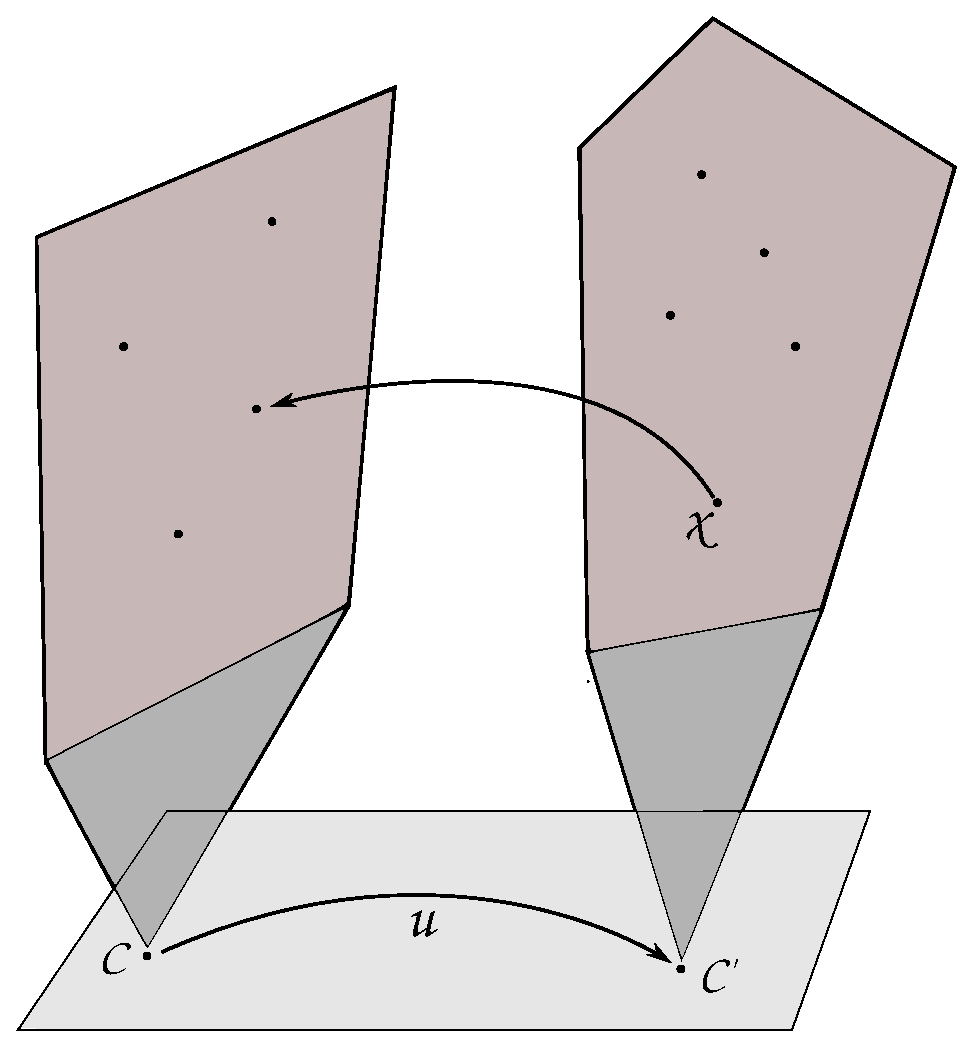
\includegraphics[width=.325\textwidth]{disegno.eps}
	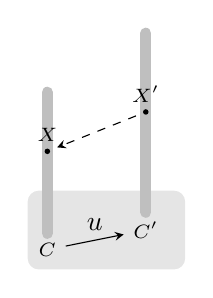
\begin{tikzpicture}[>=stealth]
		\fill[gray!20,rounded corners] (0,0) rectangle (2,1);
		\node[font=\scriptsize] (C) at  (.25,.25) {$C$};
		\node[font=\scriptsize] (C') at (1.5,.5)  {$C'$};
		\draw[->] (C) -- (C') node[above, pos=.5] {$u$};
		%
		\draw[line width=4pt, gray!50, cap=round] (C) -- +(0,2);
		\draw[line width=4pt, gray!50, cap=round] (C') -- +(0,2.5);
		%
		\fill (1.5,2) circle (1pt) node (X') {};
		\fill (.25,1.5) circle (1pt) node (X) {};
		\draw[dashed,->] (X') -- (X);
		\node[above, font=\scriptsize] at (X') {$X'$};
		\node[above, font=\scriptsize] at (X) {$X$};
	\end{tikzpicture}
\end{center}
There is of course a similar correspondence for \emph{covariant} functors; the situation is conveniently depicted by the table
\begin{center}
	\begin{tabular}{ccc}
		\textbf{name}       & \textbf{variance}   & \textbf{condition} \\ \toprule
		fibration           & $\clC\to\Set$       &
		$
			\vcenter{\tiny \xymatrix@R=5mm{
		X \ar[r] \ar@{.}[d] & X'\ar@{.}[d]                             \\ \midrule
		pX \ar[r]_f         & C'
			}}
		$
		\\ \midrule
		opfibration         & $\clC^\op \to \Set$ &
		$
			\vcenter{\tiny \xymatrix@R=5mm{
		X \ar[r] \ar@{.}[d] & X'\ar@{.}[d]                             \\ \midrule
		C \ar[r]_f          & pX'
			}}
		$
		\\ \bottomrule
	\end{tabular}
\end{center}
% \f{La notazione va uniformata a questa scelta}
\begin{corollary}\label{da_collage}
	Given a profunctor $\fkR : \clA \pto \clB$, regarded as a functor $R : \clA^\op\times \clB \to \Set$, we can consider the category of elements $\elts{\clA^\op\times\clB}{R}$; this is often called the \emph{collage} or the \emph{graph} of $R$. In this case, we denote the category $\elts{\clA^\op\times\clB}{R}$ as $\clA\uplus_R\clB$, to stress the intuition that $R$ prescribes a way to glue together two categories $\clA,\clB$ specifying a set of `fake' arrows $R(A,B)$ that consistently interact with the arrows in $\clA,\clB$ (compare with \autoref{hint_at_collage}, and with \autoref{11_ramsey} below).
\end{corollary}
\begin{remark}\label{collage_explaned}
	The above definition deserves to be expanded a little more: from \autoref{} we get that the category $\clA\uplus_R\clB$ results as the category whose objects are those of the disjoint union $\clA_o\sqcup\clB_o$, and where the hom-set $\clA\uplus_R\clB(X,Y)$ is equal to
	\begin{enumtag}{c}
		\item $\clA(A,A')$ if $(X,Y)=(A,A')$ is a pair of objects in $\clA$;
		\item $\clB(B,B')$ if $(X,Y)=(B,B')$ is a pair of objects in $\clB$;
		\item $R(A,B)$ if $X=A$ is an object of $\clA$, and $Y=B$ is an object of $\clB$;
		\item empty in every other case.
	\end{enumtag}
	From this definition, it is evident that every profunctor $\fkR : \clA \pto \clB$ gives rise via its fibration of elements to a span 
	\[ \vcenter{\xymatrix{
	& \clA\uplus_\fkR \clB \ar[dr]\ar[dl]& \\ 
	\clA  && \clB
}} \]
\end{remark}
Thus, we have obtained a concrete model for a category that realises the generalised relation between $\clA,\clB$; the structure $\clA\uplus_R\clB$ is `carved' from $\clA,\clB$ separately, starting from (semi-)free relations witnessing the fact that $\fkR$ connects $\clA,\clB$ in a weak way. For example, if $\fkR : \clA^\op\times \clB \to \Set$ is the empty functor, then $\clA\uplus_R\clB$ is just he disjoint union of $\clA,\clB$; and if $\fkR$ is the functor constant at the singleton set, then $\clA\uplus_R\clB$ is the \emph{join} of $\clA,\clB$, i.e. the category $\clA\coprod\clB$ where exactly a single new morphism is added between each and every object of $\clA$ and of $\clB$ (but not in the opposite direction).